\documentclass[11pt]{article}

% ---- packages ----
\usepackage[utf8]{inputenc}
\usepackage[T1]{fontenc}
\usepackage[margin=1in]{geometry}
\usepackage{amsmath,amssymb}
\usepackage{booktabs}
\usepackage{graphicx}
\usepackage{xcolor}
\usepackage{xspace}
\usepackage{authblk}
\usepackage[numbers,round]{natbib}
\usepackage{caption}
\usepackage[hidelinks]{hyperref}

\graphicspath{{figures/}}

% ---- macros ----
\newcommand{\dirfrac}{\texttt{dir\_frac}\xspace}
\newcommand{\Dhead}{\ensuremath{D_{\text{head}}}\xspace}
\newcommand{\contentpos}{\texttt{content\_pos\_frac}\xspace}
\newcommand{\imagmass}{\texttt{imag\_mass}\xspace}
\newcommand{\ropeimag}{\texttt{rope\_imag\_frac}\xspace}
\newcommand{\selfmatch}{\texttt{self\_match}\xspace}
\newcommand{\M}{\ensuremath{M}\xspace}
\newcommand{\MS}{\ensuremath{M_S}\xspace}
\newcommand{\MA}{\ensuremath{M_A}\xspace}
\newcommand{\Mt}{\ensuremath{M_t}\xspace}
\newcommand{\Wq}{\ensuremath{W_q}}
\newcommand{\Wk}{\ensuremath{W_k}}
\newcommand{\Rope}{RoPE\xspace}
\newcommand{\note}[1]{\textcolor{red}{[#1]}}

\title{\textbf{Fingerprint, Not Blueprint:\\
How Positional Schemes Set the Default Spectral Algebra of Attention}}
\author[1]{Li Hengyu}
\affil[1]{Institute for Solid State Physics, The University of Tokyo\\
\texttt{lihengyu@issp.u-tokyo.ac.jp}}
\date{}

\begin{document}
\maketitle

\begin{abstract}
The attention score of a head is a bilinear form $\mathrm{score}(i,j)=x_i^\top \M x_j$ in the learned QK operator
$\M = \Wq^\top \Wk$. Because \M is generally non-symmetric it carries a complex eigenspectrum --- but what kind of
fact about a head does that spectrum encode? We give a three-level answer for previous-token/induction circuits.
\textbf{Statically}, across seven pretrained models spanning three positional schemes, the strongest previous-token
heads are spectrally \emph{rotational} under \Rope and \emph{non-rotational, content-like} wherever position enters
outside QK (learned-absolute and ALiBi): the model-level separation is perfect at every top-$k$ we test (exact
permutation $p{=}0.029$; head-level $p{=}2.5{\times}10^{-5}$, descriptive), and zeroing the per-frequency \Rope
phase $\mathrm{Im}(\Mt)$ destroys induction precisely on a pre-identified previous-token head in each of three
\Rope models. \textbf{Dynamically}, over public Pythia checkpoints every head is born at the random-matrix
(Ginibre) null; the rotational signature locks in within the same checkpoint window as the behavior --- we find no
earlier predictive signature --- and the population-wide suppression that produces the final profile follows
circuit formation: the profile is a consolidated fingerprint of the algorithm, not its precursor.
\textbf{Causally, at toy scale}, no spectral channel is necessary: in controlled 2-layer training runs, constrained
training reroutes around every ban we imposed with final capability intact, but at a significant formation delay
(all four pre-registered contrasts $q_{\mathrm{BH}}{\le}0.016$), and the cost structure exposes each scheme's
\emph{default} --- forcing symmetry costs learned-absolute models $2.9\times$, while a \Rope head with a fully
symmetric static \M still routes directionally through the phase channel, a dissociation impossible under absolute
positions. Together, in the settings analyzed: \textbf{the positional scheme sets the default spectral algebra of
attention's solutions} --- a fingerprint sculpted after function, a default rather than a hard constraint.
\end{abstract}

\section{Introduction}
For a single attention head with norm-processed residual token $x\in\mathbb{R}^d$ and projections $\Wq,\Wk$, the
pre-softmax score is a bilinear form in one operator,
\begin{equation}
\mathrm{score}(i,j) = q_i^\top k_j = x_i^\top(\Wq^\top \Wk)x_j = x_i^\top \M x_j,\qquad \M=\Wq^\top \Wk \in\mathbb{R}^{d\times d}.
\end{equation}
\M is the natural, gauge-invariant object of study: the reparametrization $\Wq\!\to\!\Wq G,\ \Wk\!\to\!\Wk G^{-\top}$
leaves \M and every observable unchanged, so raw $\Wq/\Wk$ entries are gauge artifacts while functions of \M are
physical \citep{elhage2021framework}. \M is low rank ($\mathrm{rank}\le d_k$) and, crucially, \emph{generally
non-symmetric}---so it has a complex eigenspectrum.

A growing literature reads non-normal/complex spectral structure into transformers: Schur decompositions of the
residual-stream Jacobian \citep{fernando2026dynamics}, ``non-Hermitian'' operator-theoretic framings
\citep{chang2026dyson}, and symmetric/antisymmetric decompositions of the QK matrix \citep{saponati2025}; concurrent
work catalogues per-head complex eigenvalues of the attention interaction and ablates its skew/symmetric channels
against corpus perplexity \citep{jamil2026routing}. Yet the QK
operator's complex spectrum remains \emph{behaviorally unanchored} --- no random-matrix nulls, no head-function
taxonomy, no head-resolved causal tests, no positional-scheme contrasts --- and the field's discipline demands we ask
not whether the structure \emph{exists} but whether it \emph{does measurable work}. Concretely: does the
complex-eigenvalue view of \M predict head behavior that the plain symmetric/antisymmetric split does not already
capture?

We answer this at three levels: \emph{statics} across seven pretrained models --- GPT-2 small, OPT-1.3B, and
GPT-Neo-1.3B (learned-absolute positions), BLOOM-1b1 (ALiBi: position enters as a score bias, leaving QK positionally
unconstrained), Pythia-410m/1.4B ($25\%$ \Rope), and Llama-3-8B ($100\%$ \Rope, RMSNorm, GQA); \emph{dynamics} across
the public Pythia training checkpoints; and \emph{interventions} in constrained-from-scratch training runs. Our
contributions:
\begin{enumerate}\itemsep2pt
\item \textbf{A matched-null spectral framework for the QK operator} (\S\ref{sec:method}): four decompositions of the
norm-folded \M, a primary directionality metric \Dhead and its plain-split baseline \dirfrac, and---essential---a
\emph{random-orientation (Ginibre) null} against which directionality must be read (a random low-rank \M already has
$\dirfrac\approx1/\sqrt2$).
\item \textbf{Descriptive}: spectral directionality separates head function across all seven models
(\S\ref{sec:descriptive}), extending \citet{saponati2025} from training objective to head function.
\item \textbf{Causal anatomy} on GPT-2 (\S\ref{sec:causal}): the symmetric part \MS is $6.7\times$ more load-bearing
than the antisymmetric \MA; \MA is causally critical only for the canonical induction/previous-token circuit and inert
elsewhere. On GPT-2 the complex refinement \Dhead does \emph{not} beat \dirfrac.
\item \textbf{The architecture-conditional signature} (\S\ref{sec:reversal}): the strongest previous-token heads
are spectrally rotational under \Rope (top-quintile \Dhead) and non-rotational under learned-absolute \emph{and}
ALiBi positions (bottom-quartile, four models); the model-level separation is perfect at every top-$k$ tested
(exact permutation $p{=}0.029$; head-level $p{=}2.5{\times}10^{-5}$, descriptive); $d_k$ held fixed across schemes.
Aggregate partials are shown to be bulk-contaminated and unreliable for this contrast.
\item \textbf{Mechanism} (\S\ref{sec:mechanism}): a per-frequency complex decomposition ties \Dhead to the \Rope
rotational phase $\mathrm{Im}(\Mt)$; adding \Rope-phase features as controls attenuates \Dhead's advantage by
${\sim}47$--$61\%$ ($25\%$ \Rope) and ${\sim}70$--$98\%$ ($100\%$ \Rope), estimator-dependent.
\item \textbf{Causal confirmation} (\S\ref{sec:ablation}): ablating $\mathrm{Im}(\Mt)$ symmetrizes the relative-position
kernel and destroys induction on exactly the flagged heads.
\item \textbf{A checkpoint natural history} (\S\ref{sec:dynamics}): on Pythia-410m/160m (22 public checkpoints each),
all heads are born at the Ginibre null; the rotational signature locks in \emph{with} circuit formation (not before
it), and the population-wide suppression that produces the static profile follows formation --- the profile is a
consolidated fingerprint, not a precursor.
\item \textbf{Constrained-training interventions} (\S\ref{sec:intervention}): a $\{$APE, \Rope$\}\times\{$free,
sym-\M, $\mathrm{Im}(\Mt)$-suppressed$\}$ grid ($n{=}5$ seeds) shows no spectral channel is \emph{necessary}
(every arm reroutes) while every constraint carries a significant search cost that reveals the scheme's default
solution, and dissociates the static-antisymmetry and \Rope-phase channels at the weight level.
\end{enumerate}
One sentence unifies the three levels: \emph{the positional scheme sets the default spectral algebra of attention's
solutions --- a fingerprint sculpted after function, an economy of search rather than a hard constraint.}
We report the negatives (GPT-2 decorativeness; \MA's inertness away from a few heads) as plainly as the positives.

\section{Related work}
\textbf{QK circuits and weight-space interpretability.} \citet{elhage2021framework} frame $\M{=}\Wq^\top\Wk$ and
$W_{OV}$ as the two low-rank circuits and use \emph{OV} eigenvalue positivity as a copying statistic; they perform no
QK spectral analysis. \citet{millidge2022svd} find weight-SVD interpretable but report it \emph{fails} on QK---motivating
an orientation-recovering (Schur/complex) view. Our object and the OV/QK distinction follow this line; our contribution
is the QK-side, imaginary-axis, behavior-anchored analog.

\textbf{Symmetric/antisymmetric QK.} \citet{saponati2025} decompose $W_{qk}{=}M_s{+}M_n$ and define a Frobenius
symmetry score, anchoring it to the \emph{training objective}. Our \dirfrac is a monotone transform of their score
($s = 1-2\,\dirfrac^2$); we anchor the split to \emph{head function} and add the complex/Schur refinement and its
causal test.

\textbf{Non-normal / non-Hermitian transformers.} Concurrently with this work, \citet{jamil2026routing} decompose
the per-head attention interaction into skew (``routing'') and symmetric (``filtering'') channels across $1{,}776$
heads of five pretrained models, report $\max\mathrm{Re}\,\lambda>0$ for every head, find by all-heads truncation
surgery on GPT-2 Large that the symmetric channel is by far the more load-bearing (convergent, at the aggregate
level, with our \S\ref{sec:causal}), and train a stability-constrained skew-minus-diagonal attention from scratch.
Their analysis stops at norms, ranks, and stability --- no behavioral taxonomy, no random-matrix null, no
head-resolved causal test, no positional-scheme contrast, and their weight-level routing--filtering ratio is (like
Saponati's score) a monotone transform of \dirfrac --- so it cannot ask whether the complex spectrum does work
\emph{beyond} the plain split; that anchoring is our contribution. \citet{fernando2026dynamics} Schur-decompose the residual-stream
\emph{Jacobian} and show learned non-normality is functionally central---but on a different operator, without
pseudospectra, and anchored to rank/propagation, not head function. \citet{chang2026dyson} labels $\Wq^\top\Wk$
non-Hermitian in a Dyson-series theory with no computation. We differ by analyzing the QK operator's complex spectrum
empirically and anchoring it to head behavior.

\textbf{RoPE and positional heads.} \Rope \citep{su2021roformer} injects $e^{im\theta_t}$ phase,
$\theta_t=\mathrm{base}^{-2t/d}$. \citet{barbero2025rope} and \citet{urrutia2025decoupling} show positional heads use
high \Rope frequencies. We connect a \emph{weight-space} directionality scalar to per-head \Rope-frequency usage and to
head function, which they do not.

\textbf{Circuit formation over training.} \citet{olsson2022induction} established the induction phase change;
\citet{tigges2024llm} track circuits across all Pythia checkpoints behaviorally (induction at ${\sim}2{\times}10^9$
tokens); toy-model studies dissect formation \citep{bietti2023birth,reddy2024mechanistic,singh2024needs}; and
\citet{chen2024sudden} regularize an interpretable attention property during MLM pretraining --- the template our
intervention ports to autoregressive weight space. \citet{saponati2025} track their symmetry score during training
(per-layer, own encoder/decoder runs). None of these tracks a weight-space spectral quantity per head across public
checkpoints against the phase change (\S\ref{sec:dynamics}), and none constrains QK spectral structure during
autoregressive training (\S\ref{sec:intervention}).

\textbf{Constrained-attention training.} Hard symmetric (shared-QK) causal LMs exist --- Reformer
\citep{kitaev2020reformer} and recent systematic sharing studies --- and symmetric dot-product BERT trains well
\citep{courtois2024symmetric}, but none analyzes circuits under the constraint, and the soft, decomposed versions
(penalize only \MA, or only $\mathrm{Im}(\Mt)$) are new here; concurrent observational work crosses positional
schemes with induction formation in toy models \citep{huang2026dissecting}.

\textbf{Head taxonomy.} We use standard detectors---previous-token, duplicate, induction \citep{olsson2022induction}---and
IOI \citep{wang2022ioi} head classes for validation.

\section{Method}\label{sec:method}
\textbf{Object and folding.} We use TransformerLens with \texttt{fold\_ln=True} to absorb the norm gain into $\Wq,\Wk$,
and analyze the norm-folded operator $M_{\text{eff}}=C\M C$ for LayerNorm (centering $C=I-\tfrac1d\mathbf{1}\mathbf{1}^\top$)
and $M_{\text{eff}}=\M$ for RMSNorm. All spectral work is float64. We verify the convention by reconstructing the
model's own pre-softmax scores from \M and matching to $<10^{-4}$ (learned-absolute) or, for \Rope models where position
cancels only at $i{=}j$, matching the diagonal (bf16 models match to bf16 precision; the fast metric path is exact,
$\dirfrac\ \Delta{=}10^{-16}$). A random $G\in GL(d_k)$ leaves \M, its eigenvalues, and \Dhead invariant to ${\sim}10^{-14}$
while changing raw column norms---confirming gauge hygiene.

{\sloppy\textbf{Decompositions.} Per head we compute the SVD, the symmetric/antisymmetric split $\M{=}\MS{+}\MA$,
the real Schur form ($2\times2$ blocks $\to$ rotation angles $\theta$), and the complex eigendecomposition (with
eigenvector condition number as a non-normality flag).\par}

\textbf{Metrics.}
\begin{align}
\dirfrac &= \|\MA\|_F/\|\M\|_F && \text{(plain antisymmetric magnitude; Saponati's score)}\\
\Dhead &= \textstyle\sum_r |\mathrm{Im}\,\lambda_r| \big/ \sum_r |\lambda_r| && \text{(primary complex/Schur directionality)}\\
\contentpos &= \textstyle\sum \lambda^+ \big/ \sum |\lambda| \ \text{of}\ \MS && \text{(signed content axis; QK-side echo of OV positivity)}
\end{align}
plus $\text{henrici}=\sqrt{\|\M\|_F^2-\sum|\lambda|^2}/\|\M\|_F$ (departure from normality) and \selfmatch (diagonal
dominance of $W_E \M W_E^\top$).

\textbf{The random-orientation null (essential).} A random low-rank \M is already highly ``directional'': for
independent Gaussian $\Wq,\Wk$ the symmetric and antisymmetric parts get equal expected Frobenius mass, so
$\dirfrac_{\text{null}}\approx 1/\sqrt2\approx0.707$ and \Dhead's null is likewise high. We therefore report every
metric relative to a \emph{matched-$\Sigma$ random-orientation null} (same singular values, random left/right frames),
computed exactly in the rank-$k$ core. Empirically $\dirfrac_{\text{null}}{=}0.707$, $D_{\text{head,null}}{=}0.608$;
$141/144$ GPT-2 heads deviate ($|z|{>}2$ on \dirfrac or \Dhead; \dirfrac alone: $140/144$). Nulls are computed
exhaustively for GPT-2; the cross-model analyses of \S\ref{sec:reversal} use raw metrics --- on GPT-2,
null-referenced metrics give an indistinguishable partial ($-0.204$ vs $-0.206$), so this choice is not load-bearing.

\textbf{Models \& corpus.} GPT-2 small (144 heads), OPT-1.3B (768), GPT-Neo-1.3B (384), BLOOM-1b1 (384; ALiBi),
Pythia-410m/1.4B (384), Llama-3-8B (1024; GQA expanded, RMSNorm, bf16). Behavioral runs use a $1\mathrm{k}\times128$ slice of \texttt{NeelNanda/pile-10k}; detectors use repeated-random
sequences. All on one A100.

\textbf{Checkpoint and intervention pipelines.} For \S\ref{sec:dynamics} we load Pythia public checkpoints natively
(TransformerLens \texttt{checkpoint\_value}); the fused-QKV unpacking and folding conventions were verified against
the main-revision pipeline to machine precision (weight metrics at the final checkpoint match the independent
pipeline exactly, $\Delta{=}0$). For \S\ref{sec:intervention} we train 2-layer attention-only models from scratch
with soft spectral penalties; definitions and the crucial sym-\M\,$\neq$\,$\mathrm{Im}(\Mt)$ distinction are given
there. Pre-registration: the dynamics questions (Q1--Q3) and intervention predictions (P1--P4) were locked in the
project's intervention plan before any checkpoint was downloaded or any constrained run launched; we report the
falsified predictions as findings.

\section{Spectral directionality separates head function}\label{sec:descriptive}
On GPT-2 ($n{=}144$, Spearman, BH-FDR $q{<}10^{-3}$), directionality maps onto head class (Table~\ref{tab:taxonomy}).
Previous-token heads are directional (high \dirfrac, low content positivity); duplicate/similarity heads are symmetric;
\textbf{induction heads read as content-like}. We note plainly that our preregistered hypothesis predicted the
opposite (induction heads directional); that prediction \emph{failed}. The two-head-circuit reading --- the induction
head's QK consumes \emph{composed content} written by a previous-token head, so its single-head \M is symmetric ---
was recorded in the analysis plan before these correlations were computed, and we verify it directly:
by the K-composition statistic (the Frobenius overlap of an induction head's QK operator with an earlier head's OV
write, ranked over all earlier heads), \textbf{the canonical previous-token head ranks \#1 for every induction head
tested} --- GPT-2's 4.11 for 5.1/5.5/6.9 (ranks 1/60, 1/60, 1/72) and Pythia-410m's 5.2 for 8.6/10.9/11.14 (1/128,
1/160, 1/176) --- confirming that induction QK is wired to consume the prev head's composed output. \textbf{Copying (OV) is orthogonal to every QK metric}, a clean control. The content
signature is legible: \selfmatch equals \contentpos at $r{=}0.96$; empirical pre-softmax score asymmetry on real
inputs tracks \dirfrac at $0.66$. This replicates on Pythia and, attenuated, on Llama (\contentpos$\to$prev $-0.30$
vs GPT-2's $-0.63$; \S\ref{sec:reversal}), establishing spectral directionality as an architecture-general
head-function signature and extending \citet{saponati2025} from objective to function (Fig.~\ref{fig:plane}).

\begin{table}[t]\centering\small
\begin{tabular}{lcccc}\toprule
metric & prev-token & duplicate & induction & copying (OV)\\\midrule
\dirfrac      & $+0.47$ & $-0.59$ & $-0.50$ & $0.06$ (ns)\\
\contentpos   & $-0.63$ & $+0.59$ & $+0.57$ & ns\\
\imagmass     & $+0.56$ & $-0.65$ & $-0.61$ & ns\\
\bottomrule\end{tabular}
\caption{Spearman correlations of spectral metrics with head-type scores (GPT-2, $n{=}144$; all shown are
FDR-significant). Copying is an orthogonal OV-side control.}
\label{tab:taxonomy}
\end{table}

\begin{figure}[t]\centering
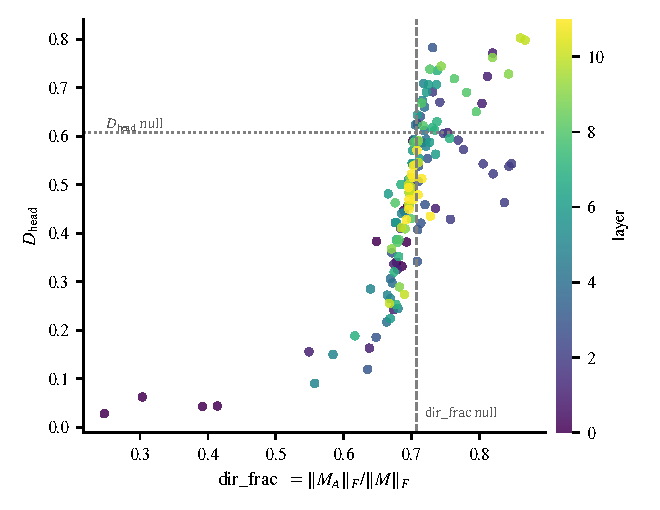
\includegraphics[width=0.6\linewidth]{gpt2_dirfrac_vs_Dhead.pdf}
\caption{The content--direction plane (GPT-2). Each point is a head; dashed lines mark the random-orientation null
$(\dirfrac_{\text{null}}{\approx}0.707,\ D_{\text{head,null}}{\approx}0.608)$. A content cluster (low on both, mostly
layer 0) sits below the null; directionality is read as deviation from it.}
\label{fig:plane}
\end{figure}

\section{Causal anatomy on GPT-2: \texorpdfstring{$\MS\gg\MA$}{MS >> MA}}\label{sec:causal}
\textbf{Symmetrization ablation.} Replacing a head's \M with \MS (killing \MA) or \MA (killing \MS) and measuring
held-out CE, the \textbf{symmetric part is $6.7\times$ more load-bearing}: $\sum \Delta\mathrm{CE}_{\text{anti}}{=}2.60$
vs $\sum\Delta\mathrm{CE}_{\text{sym}}{=}0.39$; killing \MA costs $\le0.02$ general CE anywhere. But a \emph{targeted
induction task} exposes that \MA is causally \emph{essential} for specific heads: killing it on the canonical induction
head~5.1 raises induction loss $8\times$ ($0.21\to1.77$; $15\times$ the next-largest effect) and on the previous-token
head~4.11 by ${\sim}50\%$. Canonical induction heads 5.5/6.9 show smaller positive effects ($+0.03$, ranks 7--8 of
144); the top-5 by effect are 5.1, 4.11, 6.7, 3.0, 8.5, so top-5 overlap with the canonical circuit is 2/5
(hypergeometric $p{=}0.014$), with the argmax landing on a canonical induction head --- circuit-level enrichment, not
an exact circuit match. Crucially this importance is a \textbf{discrete circuit fact}: no spectral scalar (\dirfrac,
\Dhead, \imagmass, $\|\MA\|$) predicts \emph{which} heads need \MA (all $|\rho|\lesssim0.1$), so the 144-head
aggregate is null.

\textbf{Incremental validity.} For predicting the previous-token score, the complex refinement adds no reliable
positive increment on GPT-2: $\mathrm{partial}\,\rho(\Dhead,\text{prev}\mid\dirfrac)=-0.21$ (layer-clustered 95\% CI
$[-0.51,+0.08]$ --- the point estimate is negative but not reliably so; among prev-candidate heads,
$\text{prev}{>}0.05$, the residual association is strongly negative, $-0.63$), and in a nested regression on the
ablation effect \dirfrac explains $0.001$ of variance rising only to $0.028$ with \Dhead added, the added term
wrong-signed. On learned-absolute positions, the plain antisymmetric magnitude captures everything the complex
spectrum reliably offers about its strong prev heads; \S\ref{sec:reversal} shows this head-profile pattern
generalizes to OPT-1.3B and GPT-Neo-1.3B, though their aggregate statistics do not.

\section{The architecture-conditional signature (main result)}\label{sec:reversal}
We run the incremental-validity test across positional schemes on seven models (Table~\ref{tab:reversal}). On every
\Rope model, \Dhead's incremental contribution beyond \dirfrac is positive and robust (clustered CIs
$[+0.21,+0.59]$). Under learned-absolute positions, however, the \emph{aggregate} statistic is heterogeneous
(GPT-2 $-0.21$; OPT-1.3B $+0.35$; GPT-Neo-1.3B $+0.20$) --- and decomposing it shows why it is the wrong statistic: a
positive gradation among near-zero-prev \emph{bulk} heads is present in most models (including GPT-2: $+0.25$ within
$\text{prev}{\le}0.05$), while the signal that differs by architecture lives in the \emph{strong} previous-token
heads themselves. The last column of Table~\ref{tab:reversal} gives each model's top-5 prev heads' within-model
\Dhead percentile: \textbf{bottom-quartile under learned absolute} (medians $0.21/0.23/0.14$; e.g.\ GPT-2's 4.11 at
$0.22$; all with content-like symmetric profiles, \contentpos $0.46$--$0.57$) and ALiBi ($0.26$) versus \textbf{top-quintile under
\Rope} (medians $0.89/0.85/0.79$; Fig.~\ref{fig:main}a). Holding
$d_k{=}64$ fixed (GPT-2, OPT-1.3B, Pythia-410m: $0.21/0.23$ vs $0.89$) ties the contrast to the positional scheme,
not head dimension.

\textbf{Model-level inference and sensitivity.} Heads within a model share training, layers, and detectors, so the
model is the honest experimental unit. At model level the separation is \emph{perfect} --- every non-\Rope model's
top-5 median sits below every \Rope model's --- giving an exact model-level permutation $p{=}1/\binom{7}{3}{=}0.029$,
the minimum attainable with seven models; the head-level joint Mann--Whitney $p{=}2.5{\times}10^{-5}$ is reported as
descriptive only. The contrast is not an artifact of the $k{=}5$ choice: model-level separation is perfect at every
$k\in\{1,3,5,10\}$, and leave-one-model-out preserves it for all seven models. The binding statistical limit is the
model count itself --- one ALiBi and one full-\Rope family --- which more model families, not more heads, would
address (Limitations). The defensible claim is \emph{profile-level}: \textbf{the heads that implement previous-token
attention are spectrally rotational under \Rope and spectrally non-rotational (content-like) under learned absolute
positions.} Mechanistically, this is what the positional algebra dictates: with learned absolute embeddings,
prev-token attention can be built by \emph{matching} adjacent position vectors --- a symmetric, content-like
operation --- whereas \Rope builds it from \emph{rotations}, imprinting complex eigenstructure. \textbf{ALiBi
provides the cleanest test}: position enters as a score \emph{bias}, so QK needs no positional structure at all ---
and BLOOM-1b1's top prev heads are indeed non-rotational (percentile $0.26$), patterning with the learned-absolute
group exactly as the mechanism predicts. Under \Rope these
heads sit at the \dirfrac null (${\sim}0.70$) with \Dhead at the Ginibre value (${\approx}0.61$) while the
population suppresses below it (medians $0.40$--$0.45$; per-model matched nulls: 410m prev heads' \Dhead
$z\in[-0.1,+5.0]$ vs population median $z{=}{-}11$; 1.4B prev-head median $z{=}{-}3.7$ vs population
$z{=}{-}13.9$): they \emph{retain} near-random rotational structure that other heads learn to suppress, and the
Schur/complex view detects this where the Frobenius magnitude cannot.

\textbf{Robustness and scope.} Three qualifications sharpen the claim. (i)~\emph{Metric specificity}: among
complex-spectrum summaries, \imagmass is incrementally positive on all models and Henrici non-normality negative on
all; \Dhead composites these two channels. No single aggregate scalar separates the schemes --- the head-profile
statistic does. (ii)~\emph{Class vs bulk}: the \Rope positives are class-level separation (rank-biserial
$+0.44/+0.60$ at $\text{prev}{>}0.2$ in Pythia; $+0.29$ at $\text{prev}{>}0.1$ in Llama) \emph{plus} bulk gradation;
within confirmed prev heads there is no further gradation (subset partials n.s.). Under learned-absolute positions
the class-level tests are null-to-negative at the strong end (GPT-2 $-0.39$ at $\text{prev}{>}0.2$, significant;
OPT $-0.11$ n.s.; GPT-Neo $+0.13$ n.s.), though GPT-Neo shows a positive signal at the looser $\text{prev}{>}0.1$
band ($+0.34$) driven by its moderate-prev heads --- its \emph{top} prev heads still sit at percentile $0.14$. The
learned-absolute models are thus heterogeneous in their moderate bands (candidate sources: training corpus,
GPT-Neo's alternating local-attention layers) while uniform at the top of the class. (iii)~GPT-2's negative
aggregate concentrates exactly among prev-candidate heads ($-0.63$ at $\text{prev}{>}0.05$); OPT's positive
aggregate is entirely bulk ($-0.18$ among its prev candidates). Aggregate partials should not be read as the
architecture signal in either direction.

\begin{table}[t]\centering\footnotesize\setlength{\tabcolsep}{3.5pt}
\begin{tabular}{lcccccccc}\toprule
model & $d_k$ & positions & norm & $\rho_{\texttt{dir}}$ & $\rho_{D}$ & partial & 95\% CI & \textbf{top-5 pctile}\\\midrule
GPT-2        & 64  & absolute   & LN  & $+0.47$ & $+0.29$ & $-0.21$ & $[-0.51,+0.08]$ & $\mathbf{0.21}$\\
OPT-1.3B     & 64  & absolute   & LN  & $+0.08$ & $+0.28$ & $+0.35$ & $[+0.19,+0.48]$ & $\mathbf{0.23}$\\
GPT-Neo-1.3B & 128 & absolute   & LN  & $+0.35$ & $+0.41$ & $+0.20$ & $[+0.07,+0.33]$ & $\mathbf{0.14}$\\
BLOOM-1b1    & 96  & ALiBi      & LN  & $+0.13$ & $+0.25$ & $+0.34$ & $[+0.22,+0.47]$ & $\mathbf{0.26}$\\
Pythia-410m  & 64  & \Rope 25\% & LN  & $+0.57$ & $+0.62$ & $+0.35$ & $[+0.21,+0.47]$ & $\mathbf{0.89}$\\
Pythia-1.4B  & 128 & \Rope 25\% & LN  & $+0.31$ & $+0.60$ & $+0.50$ & $[+0.38,+0.59]$ & $\mathbf{0.85}$\\
Llama-3-8B   & 128 & \Rope 100\%& RMS & $+0.32$ & $+0.38$ & $+0.33$ & $[+0.21,+0.45]$ & $\mathbf{0.79}$\\
\bottomrule\end{tabular}
\caption{Incremental validity of \Dhead over \dirfrac for the previous-token score, seven models / three
positional schemes. $\rho_{\texttt{dir}}=\rho(\dirfrac,\text{prev})$, $\rho_D=\rho(\Dhead,\text{prev})$; partial $=
\mathrm{partial}\,\rho(\Dhead,\text{prev}\mid\dirfrac)$ (Spearman of OLS residuals); CIs: layer-clustered bootstrap
(heads share layers/training, design effects $3.6$--$6.9$; Llama heads additionally share K-projections within GQA
groups of 4). \textbf{The aggregate partial is heterogeneous under learned-absolute positions} ($-0.21/+0.35/+0.20$)
because it mixes a near-ubiquitous positive bulk gradient (among near-zero-prev heads) with the class-level signal;
\textbf{the architecture-conditional statistic is the last column} --- the median within-model \Dhead percentile of
the top-5 previous-token heads: bottom-quartile under learned-absolute and ALiBi vs top-quintile under \Rope (perfect model-level separation,
exact permutation $p{=}0.029$; head-level $p{=}2.5{\times}10^{-5}$, descriptive). $d_k{=}64$ is shared by GPT-2, OPT-1.3B, and Pythia-410m, so the contrast
tracks the positional scheme, not head dimension. All \Rope partials survive BH-FDR.}
\label{tab:reversal}
\end{table}

\begin{figure}[t]\centering
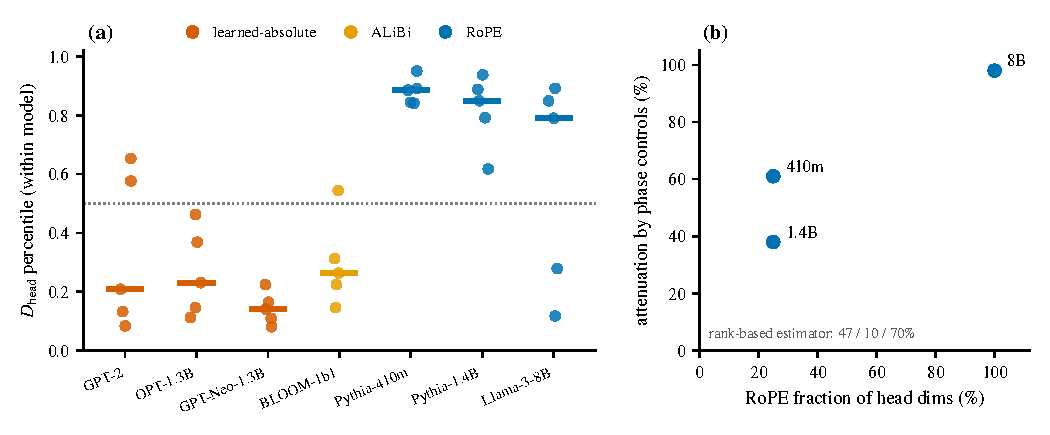
\includegraphics[width=\linewidth]{paper_main_result.pdf}
\caption{\textbf{(a)} Within-model \Dhead percentile of each model's top-5 previous-token heads: bottom-quartile
under learned-absolute (red) and ALiBi (orange) positions, top-quintile under \Rope (blue); joint
Mann--Whitney $p{=}2.5{\times}10^{-5}$; bars mark per-model medians. \textbf{(b)} Attenuation of \Dhead's
advantage by \Rope-phase controls grows with \Rope fraction (hybrid estimator: $61\%/38\%$ at $25\%$, ${\sim}98\%$ at
$100\%$; see Table~\ref{tab:mediation} for estimator sensitivity --- with two dose levels this is suggestive, not an
established dose--response).}
\label{fig:main}
\end{figure}

\section{Mechanism: \texorpdfstring{\Dhead}{Dhead} tracks the RoPE phase}\label{sec:mechanism}
\Rope pairs each head's $d_k$ dims (rotate-half convention, verified) into frequencies $\theta_t$; the QK interaction
per frequency is a rank-1 complex sub-operator $\Mt=w_q^t\,\overline{w_k^t}^{\top}$, with the static
$\M=\sum_t\mathrm{Re}(\Mt)$. The \emph{directional} (relative-position-asymmetric) content is carried by the imaginary
part:
\begin{equation}
\mathrm{score}(\Delta)-\mathrm{score}(-\Delta)=\sum_t 2\sin(\Delta\theta_t)\,n^\top \mathrm{Im}(\Mt)\, n .
\end{equation}
(Full-score reconstruction from $\{\Mt,\theta_t\}$ matches the model to $10^{-6}/10^{-2}$ in fp32/bf16.) Empirically,
previous-token heads have high rotary directional fraction \ropeimag (correlation with prev: $+0.53/+0.42/+0.50$ for
410m/1.4B/Llama) concentrated at \emph{high frequencies} ($+0.68$ on full-\Rope Llama---a
\citet{barbero2025rope,urrutia2025decoupling} replication), and \textbf{\Dhead tracks this deployment}. Adding per-frequency \Rope-phase summaries as controls \emph{attenuates}
\Dhead's residual association substantially (Table~\ref{tab:mediation}) --- most completely on full-\Rope Llama,
where the default-estimator residual is indistinguishable from zero ($+0.006$, $p{=}0.84$; fully rank-based:
$+0.075$, $p{=}0.016$). Two qualifications. First, all quantities are co-derived from the same weights, so this is
shared-variance accounting, not causal mediation. Second, the attenuating covariate \emph{changes identity} with
\Rope fraction: on partial-\Rope Pythia the attenuation runs through \ropeimag (how \emph{much} rotary content is
directional; \texttt{freq\_centroid} alone attenuates nothing, $+0.35$), whereas on full-\Rope Llama it runs almost
entirely through \texttt{freq\_centroid} (\emph{where in frequency} the directional mass sits: alone
$+0.33\to-0.00$, while \ropeimag alone leaves $+0.32$) --- consistent with all directional content being rotary by
construction at $100\%$, shifting the informative axis from amount to location. The pattern is consistent with
fuller attenuation at higher \Rope fraction, but with two dose levels and within-dose spread ($61\%$ vs $38\%$)
comparable to the dose gap, we do not press a dose--response reading. The relative-position kernel confirms these
heads peak at $\Delta{=}{-}1$ with \Rope-periodic oscillation (Fig.~\ref{fig:kernels}, left).

\textbf{Placebo controls.} Two controls calibrate what the attenuation means. \emph{(i) \Rope-model specificity:} on
all three learned-absolute models (no \Rope), computing a pseudo-\ropeimag with a fake rotate-half pairing over all
head dims yields no prev signal (GPT-2 $-0.14$, OPT-1.3B $-0.06$, GPT-Neo-1.3B $-0.09$; all n.s., vs
$+0.42$--$+0.53$ on \Rope models), and adding the pseudo-phase features barely attenuates ($4$--$22\%$): the recipe
finds nothing where \Rope is absent. \emph{(ii) Pairing
specificity:} randomly permuting the rotary columns of $W_Q,W_K$ --- which leaves \M (hence \Dhead, \dirfrac)
unchanged and preserves rotary-\emph{block} membership, but scrambles the pairing and frequency assignment --- still
attenuates $31$--$38\%$ on average, so much of the attenuation is carried by rotary-block membership alone. The
increment specific to the \emph{true} pairing/frequency assignment is marginal on Pythia-410m (true $60.7\%$ vs the
permutation null, empirical $p{=}0.039$, $n{=}50$ permutations) and not significant on Pythia-1.4B ($37.7\%$,
$p{=}0.12$). The mechanism is thus \Rope-specific and largely block-level; the finer pairing-level reading should be
held lightly.

\begin{table}[t]\centering\footnotesize\setlength{\tabcolsep}{4pt}
\begin{tabular}{lccccc}\toprule
model & \Rope frac. & partial & $+$phase controls & atten.\ (hybrid) & atten.\ (rank)\\\midrule
Pythia-410m & $25\%$  & $+0.35$ & $+0.14$ & $61\%$ & $47\%$\\
Pythia-1.4B & $25\%$  & $+0.50$ & $+0.31$ & $38\%$ & $10\%$\\
Llama-3-8B  & $100\%$ & $+0.33$ & $+0.006$ ($p{=}0.84$) & ${\sim}98\%$ & $70\%$\\
\bottomrule\end{tabular}
\caption{Attenuation of \Dhead's residual prev-token association (partial $=\mathrm{partial}\,\rho(\Dhead,
\text{prev}\mid\dirfrac)$) when per-frequency \Rope-phase summaries
(\ropeimag, \texttt{freq\_centroid}) are added as controls. ``Hybrid'' is the paper's default estimator (Spearman of
OLS residuals); ``rank'' is fully rank-based, under which the Llama residual is small but nonzero ($+0.075$,
$p{=}0.016$). All quantities are deterministic functions of the same weights: this is shared-variance accounting
among co-derived features, \emph{not} causal mediation.}
\label{tab:mediation}
\end{table}

\section{Causal confirmation: ablating \texorpdfstring{$\mathrm{Im}(\Mt)$}{Im(Mt)}}\label{sec:ablation}
We ablate a head's directional \Rope content by zeroing $\mathrm{Im}(\Mt)$ (dropping the $\sin(\Delta\theta)$
component), which \textbf{symmetrizes} its relative-position kernel; the decomposition
$\text{full}=\text{symmetric}+\text{directional}$ is verified to $6\times10^{-6}$ (fp32; $2\times10^{-5}$ on bf16
Llama). Sweeping the ablation over \emph{all} heads of all three \Rope models, the largest induction-loss effect
lands \textbf{on a top-2 prev-scoring head every time} --- an identity predicted a priori: Pythia-410m head~5.2
(prev rank 1/384; prev~$0.95$, $\Dhead\,0.61$): induction CE $0.52\to2.24$ (${\sim}4\times$; exact permutation
$p{=}1/384$); Pythia-1.4B head~1.11 (rank 1/384): $0.56\to1.11$ (${\sim}2\times$; $p{=}1/384$); Llama-3-8B
head~L14.H26 (rank 2/1024; prev~$0.65$, $\Dhead\,0.61$): $0.30\to0.91$ (${\sim}3\times$; $p{=}2/1024$) --- jointly
${\approx}10^{-8}$ under random assignment. (Llama's \#1 prev head sits in layer~0, too early to feed induction;
the causally-critical head is the mid-depth prev head.) Effects are highly concentrated: $92$--$99\%$ of heads move
by $|\Delta\text{Ind}|<0.01$; the \emph{other} $\text{prev}{>}0.5$ heads show ${\approx}0$ effects (consistent with
redundancy across a multi-head circuit), and a few low-prev heads show small effects ($\le0.17$), suggesting
downstream circuit participation the prev detector does not capture; head-level aggregate correlations are
correspondingly null. The before/after kernel shows the $\Delta{=}{-}1$ peak flattening
(Fig.~\ref{fig:kernels}, right). As in \S\ref{sec:causal}, causal importance is concentrated, not a smooth spectral
gradient; what the ablation establishes is an \emph{existence-with-predicted-identity} claim: the rotational phase
\Dhead reads is causally load-bearing for positional routing in the specific heads that carry it.

\begin{figure}[t]\centering
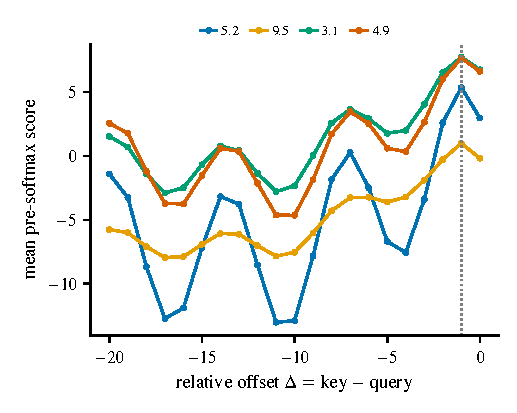
\includegraphics[width=0.49\linewidth]{pythia-410m_relpos_kernel.pdf}\hfill
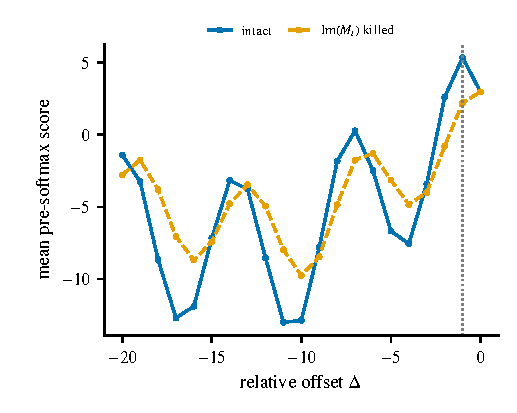
\includegraphics[width=0.49\linewidth]{pythia-410m_ablate_kernel_5_2.pdf}
\caption{\textbf{Left:} corpus-averaged relative-position score kernels of top previous-token heads (Pythia-410m) peak
at $\Delta{=}{-}1$ with \Rope-periodic oscillation. \textbf{Right:} ablating $\mathrm{Im}(\Mt)$ on the induction-feeding
head~5.2 flattens the $\Delta{=}{-}1$ peak (and raises induction loss $4\times$).}
\label{fig:kernels}
\end{figure}

\section{When the imprint arises: a checkpoint natural history}\label{sec:dynamics}
The static profile (\S\ref{sec:reversal}) is an end-state. To see how it arises we track 22 public checkpoints each
of Pythia-410m and Pythia-160m (log-spaced steps $0\ldots143{,}000$; the dense early grid straddles the induction
onset at ${\sim}2{\times}10^9$ tokens \citep{tigges2024llm}), measuring per head: the audited weight metrics
(\dirfrac, \Dhead, \ropeimag), behavioral previous-token and prefix-matching scores, an in-context-learning proxy
(second-copy minus first-copy NLL on repeated-random sequences), and the K-composition wiring between each model's
eventual prev head and its induction heads. (The ``eventual prev head'' is identified retrospectively at the
final checkpoint; Q3 below tests --- and rejects --- its prospective identifiability.)

\textbf{A three-act history at half-doubling checkpoint resolution, replicated across both models}
(Fig.~\ref{fig:dynamics}).
\emph{Act I (0--0.5B tokens): silence at the null.} Every head sits at the Ginibre null (behavior $0.01$;
\ropeimag $0.500$; population median \Dhead $0.61$; K-composition at baseline) --- step 0 doubles as an in-vivo
verification of the paper's random-orientation null. \emph{Act II (1--4B tokens): sharp formation.} Previous-token
behavior jumps first ($0.37$ at step 512 $\to$ $0.95$ at step 1000 --- the same steps, and even the same $0.37$
waypoint, in both models), with induction behavior, the ICL proxy, and the K-composition wiring following within the
same window. The prev head's \emph{within-model rotary-phase (\ropeimag) percentile} snaps from at-or-below chance ($0.03$--$0.04$
at step 512, mid-formation, in both models) to the top decile ($0.90$--$0.99$) by step 1000: the signature locks in
\emph{with} the behavior --- at our half-doubling resolution, neither leads. \emph{Act III (4--300B tokens): slow
differential sculpting.} The population median \Dhead is suppressed well below the null ($0.61\to0.395$ / $0.453$)
over the next $100\times$ of training while the circuit heads retain it, and the absolute rotary-phase content of
the prev head consolidates slowly ($0.500\to0.578$, same endpoint in both models). The static ``retain-vs-suppress''
profile of \S\ref{sec:reversal} is therefore the end state of a post-formation differentiation process.

\textbf{Pre-registered answers.} Q1 (lead/lag): the percentile signature is \emph{simultaneous} with formation; the
absolute consolidation \emph{lags}. Q2: population suppression is a post-formation process. Q3 (predictive
signature): \textbf{no} --- before formation the eventual prev head is not reliably identifiable from its spectrum
(its percentile even sits low mid-formation); we report this pre-registered negative plainly. The natural history
thus bounds what statics can claim: the rotational imprint is the fingerprint the algorithm leaves in weight space,
consolidated after function --- and because observation cannot order structure and function within the formation
window, necessity can only be settled by intervention.

\begin{figure}[t]\centering
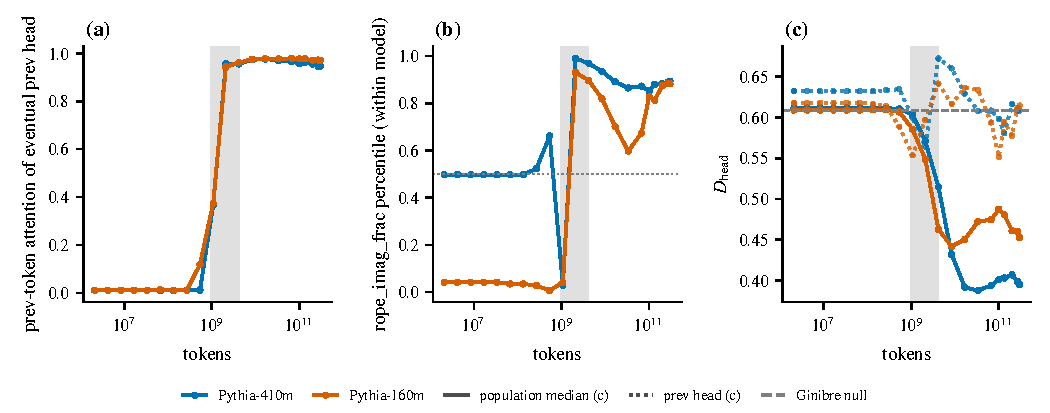
\includegraphics[width=\linewidth]{ckpt_dynamics_2models.pdf}
\caption{Checkpoint natural history, Pythia-410m (blue) and 160m (red); grey band = the formation window
($1$--$4\times10^9$ tokens). \textbf{(a)} previous-token behavior forms sharply and identically in both models.
\textbf{(b)} the prev head's \ropeimag\ percentile locks in \emph{with} behavior, not before. \textbf{(c)} the
population median \Dhead is suppressed below the Ginibre null only \emph{after} formation.}
\label{fig:dynamics}
\end{figure}

\section{Is the rotational channel necessary? Constrained-training interventions}\label{sec:intervention}
We train 2-layer attention-only models (d${=}128$, 4 heads, $d_k{=}32$) from scratch on a per-sequence random-map
task --- $x_{t+1}=f_{\mathrm{seq}}(x_t)$ w.p.\ $0.9$, uniform noise w.p.\ $0.1$, with $f_{\mathrm{seq}}$ resampled
every sequence --- which forces induction (no global memorization; no fixed-offset shortcut) and yields a crisp
formation time. Grid: $\{$APE, \Rope$\}\times\{$free; sym-\M: penalize $\|\MA\|_F^2/\|\M\|_F^2$;
$\mathrm{Im}(\Mt)$-suppressed (\Rope only): penalize $\sum_t\|\mathrm{Im}(\Mt)\|_F^2/\sum_t(\|\mathrm{Re}\|^2{+}
\|\mathrm{Im}\|^2)\}$, $n{=}5$ seeds. A load-bearing algebraic point shapes the grid: \textbf{symmetrizing the
static \M does not zero $\mathrm{Im}(\Mt)$} (the static operator contains only the $\mathrm{Re}$ parts,
$\M=\sum_t\mathrm{Re}(\Mt)+\M_{\text{non-rot}}$), so the two constraints dissociate the static-antisymmetry and
phase channels. Both penalties enforce hard (final $\mathrm{Im}$ share $0.000$; \dirfrac $0.004$--$0.006$) and no
arm loses final capability (all reach the task floor with strong prev and induction heads).

\textbf{Results against the pre-registered predictions} (Fig.~\ref{fig:intervention};
Table~\ref{tab:intervention}). P1 (free base rates) holds: APE forms fastest ($600\pm0$ steps), \Rope free at
$940\pm55$. P2's strong form is \textbf{falsified}: suppressing the phase to zero delays formation only
${\sim}1.4\times$ and the circuit \emph{reroutes} --- the prev head re-forms with $\ropeimag{=}0.005$ and a
qualitatively different (cos-only) relative-position kernel whose peak still lands at $\Delta{=}{-}1$. P3 is
\textbf{falsified in the opposite direction, our largest surprise}: forcing symmetry on APE is the \emph{costliest}
constraint in the grid ($600\to1740\pm241$, $2.9\times$) --- the fast APE solution is \emph{antisymmetric}
embedding-matching, and the symmetric variant (nearby-kernel $+$ causal mask), while reachable, is much harder to
find; trained learned-absolute LLMs end at symmetric profiles (\S\ref{sec:reversal}) with $1000\times$ more data,
and the toy exposes the search cost of that end state. P4's formation-time version fails (RoPE+sym delays
$1.66\times$) but its \textbf{mechanistic dissociation lands exactly}: the sym-arm's prev head carries
\emph{full} phase content ($\ropeimag\ 0.52$) through a \emph{fully symmetric} static operator
($\dirfrac\ 0.004$--$0.005$), and its positional kernel is indistinguishable from the free arm's --- directional
attention through a symmetric \M, which is impossible under absolute positions.

\begin{table}[t]\centering\small
\begin{tabular}{lcccc}\toprule
pre-registered contrast (formation delay) & MWU exact $p$ & $q_{\mathrm{BH}}$ & rank-biserial & HL shift\\\midrule
P1\ \ \Rope free $>$ APE free          & $0.0040$ & $0.016$ & $+1.00$ & $+300$ steps\\
P3\ \ APE sym-\M $>$ APE free          & $0.0040$ & $0.008$ & $+1.00$ & $\mathbf{+1200}$ steps ($2.9\times$)\\
P4\ \ \Rope sym-\M $>$ \Rope free      & $0.0040$ & $0.005$ & $+1.00$ & $+600$ steps\\
P2\ \ \Rope Im-sup $>$ \Rope free      & $0.0079$ & $0.008$ & $+0.92$ & $+400$ steps\\
\bottomrule\end{tabular}
\caption{Constrained-training formation delays ($n{=}5$ seeds per cell; one-sided exact Mann--Whitney, BH-FDR over
the four pre-registered contrasts). Every constraint delays formation significantly; none blocks it.}
\label{tab:intervention}
\end{table}

\begin{figure}[t]\centering
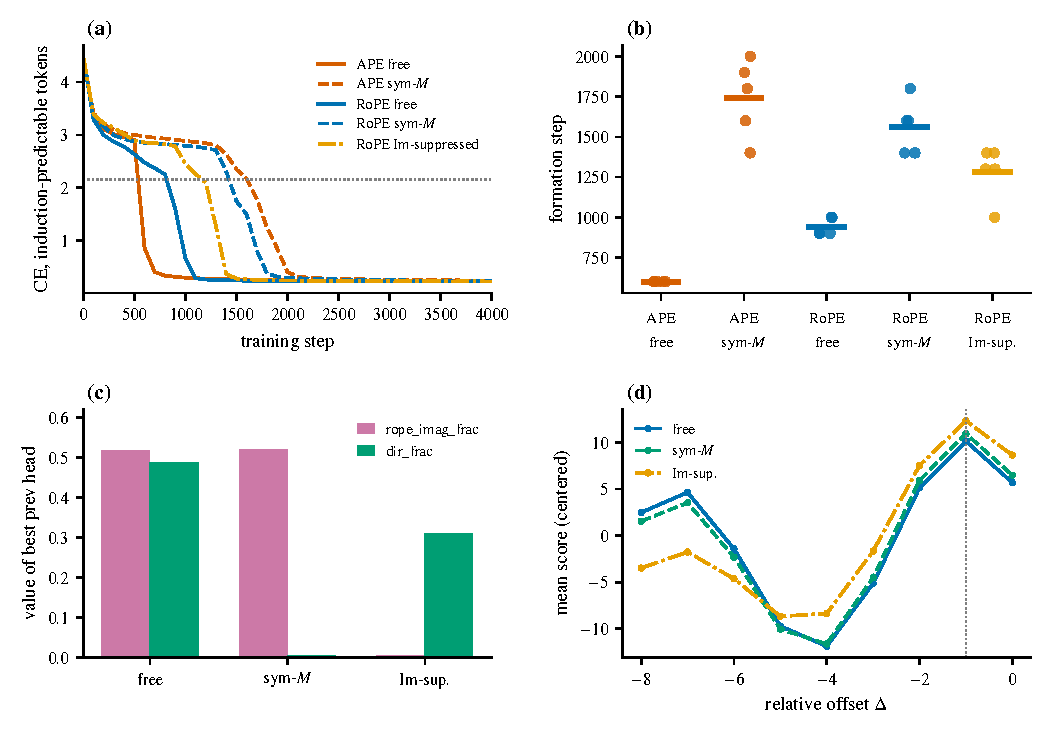
\includegraphics[width=\linewidth]{trainB_main.pdf}
\caption{Constrained-training interventions. \textbf{(a)} induction-capability curves: every arm reaches the floor;
constraints delay the drop. \textbf{(b)} formation times ($n{=}5$). \textbf{(c)} the dissociation: under sym-\M the
prev head keeps full phase content (\ropeimag) with a fully symmetric static \M (\dirfrac${\approx}0$); under
Im-suppression the reverse. \textbf{(d)} positional kernels: sym-\M is indistinguishable from free (the kernel is
carried by the untouched phase); Im-suppression reshapes the kernel but its peak stays at $\Delta{=}{-}1$
(reroute).}
\label{fig:intervention}
\end{figure}

\textbf{Verdict.} No spectral channel is \emph{necessary} --- the solution space is degenerate and training reroutes
around every constraint we imposed --- but each constraint carries a significant, quantifiable search cost
(Table~\ref{tab:intervention}), and the cost structure identifies each scheme's \emph{default} solution. With
\S\ref{sec:causal} and \S\ref{sec:ablation} this completes a three-way distinction the field often conflates:
\emph{trained-circuit dependence} (post-hoc ablations are catastrophic), \emph{developmental preference} (defaults
are found much faster), and \emph{necessity} (nothing here is strictly necessary). A companion note
\citep{li2026steering} tests the constructive converse --- ban-free \emph{assistance} --- and finds it selects the
same implementations far more cheaply than banning them ($1.3\times$ vs.\ $2.9\times$ for the antisymmetric-to-symmetric
flip) while solution-specific initialization accelerates formation outright, evidence that this spectral economy is
not only priced but steerable.

\section{Discussion}
\textbf{What earns its keep, and where.} The plain symmetric/antisymmetric split of \M is an architecture-general
descriptor of head function (\S\ref{sec:descriptive}) and, causally, the symmetric part is the workhorse
(\S\ref{sec:causal}). The \emph{complex-eigenvalue refinement} is architecture-conditional at head level: the previous-token solution is
spectrally non-rotational (content-like) under learned-absolute positions and rotational under \Rope, where \Dhead
tracks the rotational phase whose causal load \S\ref{sec:ablation} establishes head-locally
(\S\ref{sec:reversal}--\ref{sec:ablation}). This gives the recent ``non-Hermitian transformer'' program a concrete,
controlled home---the complex structure of the \emph{QK operator} does measurable, causal work precisely when position
is encoded as complex phase---while honestly bounding it: on GPT-2 the non-Hermitian label is decorative.

\textbf{Practical reading.} For weight-only head triage: under \Rope, \ropeimag\ (or the \Dhead percentile) flags
positional-routing heads without a forward pass; under absolute/ALiBi schemes the same statistics are
\emph{misleading in aggregate} (bulk gradients) and only the strong-head profile is informative. For
interpretability methodology, the dynamics result is a caution: a clean static weight--function correspondence
need not be predictive during training, and post-hoc ablation severity must not be read as developmental necessity.

\textbf{Companion work (context only).} Companion work in preparation analyzes the \emph{iterated} attention
propagator with pseudospectral tools under mask-structure nulls; none of this paper's claims relies on it. We flag
two of its directions as context: a division of labor consistent with our tool choice (eigenvalue-level summaries
suffice for the static scoring form; resolvent-level tools are needed for the depth-iterated propagator), and a
state-dependent character of induction heads that static weight fingerprints cannot capture --- consistent with
their content-like static profile in \S\ref{sec:descriptive}.

\textbf{Limitations.} (i)~The \Rope evidence in \S\ref{sec:reversal}--\ref{sec:mechanism} is correlational
(shared-variance) over heads; \S\ref{sec:ablation} supplies causation but as a concentrated per-head effect (now on
all three \Rope models). (ii)~Three learned-absolute models are tested with a consistent strong-head profile but heterogeneous aggregate and
moderate-band statistics, whose sources (training corpus; GPT-Neo's alternating local attention) are unresolved; the ALiBi scheme is covered
by a single model (BLOOM-1b1). (iii)~Inference treats heads as units: heads share layers and training (layer-clustered
design effects $3.6$--$6.9$; we report clustered CIs), and Llama heads share K-projections within GQA groups of 4
(between-group variance $0.55$--$0.79$) --- group-level dependence is only partially resolved. (iv)~Llama runs in
bf16 (float64 metrics from bf16 weights are exact w.r.t.\ the model; the diagonal convention check matches to bf16
precision only). (v)~Single-head ablations miss composition; the prev$\to$induction wiring is verified by K-composition
(\S\ref{sec:descriptive}) but full path patching is future work.
(vi)~QK biases lie outside \M and are held fixed in ablations; the prev-detector's bulk-ordering reliability is
unquantified. (vii)~A non-Llama full-\Rope family
(Qwen/Mistral) would broaden the third architecture point.

\section{Conclusion}
For the attention QK operator, the plain antisymmetric split describes head function architecture-generally; the
complex-eigenvalue refinement earns its keep only under \Rope, where it tracks the rotational phase whose causal
load head-level ablations establish. Tracking training shows this spectral signature is born at the random-matrix null, locks in with circuit
formation, and is sculpted into today's profiles after function arrives; constrained training shows it is a
\emph{default}, not a necessity --- every spectral channel we blocked was rerouted around, at a significant and
interpretable search cost. The non-Hermitian view of attention is neither uniformly profound nor uniformly
decorative: \emph{the positional scheme sets the default spectral algebra of attention's solutions}, and we
measure that claim statically, dynamically, and causally in the settings analyzed. Scaled constrained pretraining
is its direct falsification path.

\paragraph{Reproducibility \& pre-registration.}\sloppy Code in \texttt{src/}: \texttt{extract}, \texttt{decompose},
\texttt{metrics}, \texttt{observables}, \texttt{semantics}, \texttt{p4\_rope}, \texttt{rope},
\texttt{p5\_rope\_ablation}, \texttt{p9\_checkpoint\_dynamics}, \texttt{p10\_training\_intervention}. Per-head
tables: \texttt{results/cache/*\_head\_full.parquet}; checkpoint trajectories and training histories under
\texttt{results/cache/}. The dynamics questions (Q1--Q3) and intervention predictions (P1--P4) were pre-registered
in the project plan before data collection; falsified predictions (Q3, P2-strong, P3, P4-timing) are reported as
such. The full artifact bundle --- code, per-head tables, checkpoint trajectories, training histories, figure
scripts, and the pre-registration documents --- is released at
\url{https://github.com/HengyuLi-Ozaki-lab/qk-spectral-fingerprint}; the repository's version history stamps
which analyses were specified before their data existed.

\bibliographystyle{plainnat}
\bibliography{references}

\end{document}
